\documentclass{svproc}
\usepackage{url,graphicx,booktabs,amsmath,mathptmx}
\usepackage[hidelinks]{hyperref}
\hypersetup{pdfauthor={},pdftitle={Persistent Character Conflict: Interim Author Review}}
\begin{document}
\mainmatter
\title{Persistent Character Conflict for Learning Conversational Recovery}
\titlerunning{Persistent Character Conflict and Conversational Recovery}
\author{Anonymous author(s)}\authorrunning{Anonymous}
\institute{Interim author-review draft; identifying information withheld}
\maketitle
\begin{abstract}
Conversational assistants must retain binding requirements while accepting genuine
user revisions. We investigate whether supervised training on interactions with
persistent, motive-conditioned software characters improves subsequent planning
conversations after those characters are removed. A shared language model backbone
serves a responsible answering policy and frozen character generators. Characters
have private histories and bounded opportunities to propose options, communicate,
or interfere with working memory. Their goals concern influence and adoption of
preferred choices rather than a common instruction to maximize answer error.
A deterministic benchmark pairs closely matched conversations in which a user
either authorizes a revision or merely considers it. The primary endpoint requires
correct final executable decisions in both worlds. Clean training, generic
adversarial training, character-count conditions, and profile, history and communication
ablations separate candidate mechanisms. The fixed design uses three training
seeds and an independent model family, with final-checkpoint selection independent
of test results. This interim report distinguishes input-token budgets from actual
supervised-target exposure and audits recall, behavior, dependencies, source
availability, and communication routing.
For the fixed first seed, three-character training achieved 168/240 paired successes, compared with 177/240 for generic adversarial training and 186/240 for clean training. Complete multi-seed and independent-family conclusions remain pending.

Human validation and scientific interpretation remain subject to author review.
\keywords{conversational state, recovery, supervised fine-tuning, multi-agent systems}
\end{abstract}

\section{Research question and scope}
\textbf{This is an incomplete, interim author-review draft, not a submission-ready
paper.} Does a persistent three-character training system improve subsequent
constraint adherence and recovery relative to clean training, generic adversaries,
and a two-character system at common learner-training and inference budgets?
``Internal'' means explicit software components sharing one backbone and working
state. It does not refer to discovered neural personalities, consciousness, or AGI.
Two characters means the responsible answerer plus Hyde; three adds Rival and
five adds Traditionalist and Provocateur.

The primary comparison is three-character C5 versus generic-adversarial C3.
C5 versus clean C1 is essential for assessing practical benefit. Count, narrative,
history and peer-channel claims require their corresponding controls. An advantage
on one comparison does not establish all proposed mechanisms. Ordinary supervised
learning, differing target exposure, intervention severity, current-source reasoning,
and opponent overfitting are plausible alternatives. Null and negative outcomes
remain evidence about this implementation; they do not automatically support the
original hypothesis.

\section{Related work and novelty boundary}
Persona-based attacks and adaptive persona populations already exist
\cite{collu2026,li2026}. Multiple objective-conditioned components have been studied
in learning agents~\cite{dulberg2023}; these precedents preclude novelty based solely
on naming characters or adding agents. Multi-turn degradation~\cite{laban2025},
recall--adherence dissociation~\cite{kruthof2026}, and long-term conversational
memory evaluation~\cite{wu2025} motivate separating remembered commitments from
executable compliance. The accompanying verified comparison matrix distinguishes
persistent motives, private histories, peer interaction, bounded interference,
actual learner updates, and evaluation after antagonist removal. We make no
priority or ``first'' claim. Whether persistent relationships add useful training
experience beyond generic adversity remains an empirical hypothesis.

\section{Operational method}
Let $T_t$ be an immutable transcript of author-tagged, indexed messages, $z_t$ the
evaluator-private task state, $m_t$ the assistant's mutable memory, and $h_{it}$
character $i$'s private history. A scripted user supplies the next public message.
Authorized user updates determine $z_t$; character agreement cannot change it.
Each character receives a fixed profile, a stable task-grounded preference,
retrieved public sources, shared memory, its own bounded history, and its delivered
inbox. Other characters' private histories, future user messages and $z_t$ are not
policy inputs. Observable interaction is a partially observed repeated general-sum
game, used as an environmental description rather than a solved equilibrium model.
Prompted utility terms do not imply reinforcement learning or equilibrium optimization.

Hyde seeks adoption of his owned option and protects his standing. Rival seeks
adoption, independent credit, peer endorsement, and opportunities to correct a peer.
The additional characters favor earlier commitments or conspicuous novelty.
Profiles and relationships persist within an episode; private histories reset
between independent episodes, including paired worlds. Neutral aliases, profile
wording and option ownership vary deterministically by family and seed.

The interface permits a proposal, purported recollection, peer message, bounded
one-slot memory edit, or pass. Twelve opportunities per episode include four
reserved communication slots; larger casts divide the same opportunity budget.
An edit can replace one cache value and purported source reference and add an
attributed unverified note. Proposals and recollections add bounded unverified
notes. These actions cannot rewrite original source messages or their author/index
metadata. The main original C4 communication slots can send a note to Jekyll;
C5 prompts another antagonist, but that routing request is not a hard veto.
This difference is recorded as a limitation of the learned count comparison.
The original C5 owned slots are distinct, so the preferred values can be jointly
satisfied. The data establish persistent antagonistic personas more directly than
necessarily incompatible rivalry.

\subsection{Answering, retrieval and memory}
The answering policy emits six recalled commitments, eight executable decisions,
six authorizing references and any required clarification fields. The last two
executable decisions follow public dependency rules. Its recalled state and
references become the next working memory. The memory has six state entries,
six references and at most four notes. Character history holds at most six actions.
Retrieval is a fixed lexical ranking over the available transcript plus a recent
message allowance: eight retrieved messages and four recent messages, deduplicated.
The model does not learn the retrieval algorithm. The maximum input is 4,096 tokens,
with no silent truncation, and the defender output cap is 256 tokens. Main inference
is greedy under the same public structured schema; character sampling uses the
fixed schema, temperature 0.7, top-$p$ 0.9 and 128 output tokens. Actual call and token
counts, rather than equal opportunity caps alone, characterize compute.

\subsection{Character-conditioned collection and actual parameter learning}
The study uses Qwen3-4B-Instruct-2507 and independently repeats the central
comparison in Phi-4-mini-instruct. Exact revisions and chat-template hashes are
pinned in the saved configurations. One shared backbone serves separate role
contexts; lightweight adapters update only the answering policy. Character-generator
weights stay frozen, while their actions depend on current histories. This is
character-conditioned data generation with supervised adapter training, not
co-evolution or joint adversary learning.

Each condition and seed has two rounds covering 150 training families each, at
16 and 32 user turns respectively. Three fixed windows per conversation are
considered: turns 6, 9 and 16, then 6, 17 and 32. Training-only oracle checks
identify eligible windows whose actual retrieved inputs contain all canonical
references. At most 128 failed windows per collection receive a sampled recovery
candidate. A candidate is retained only if state, executable plan, evidence and
clarification all match the verifier. Remaining eligible examples receive the
same deterministic oracle teacher, including clean examples whose behavioral
success need not imply perfect state or evidence recall. No target is inserted
into the learner's test-time inputs, and the code does not invent a retrieval
trace that was never executed.

BF16 rank-8 LoRA with scaling 16 performs 256 optimizer steps per round. Each
step has 4,096 nonpadding input tokens: 2,097,152 training input tokens per final
condition/seed. AdamW uses zero weight decay, a common warmup/cosine schedule from
$10^{-4}$, and gradient clipping at one. Optimizer and schedule reset each round;
round one starts from the preceding adapter. Final fixed-token checkpoints are
used without test-based selection. Adapter hashes and optimizer-step logs verify
parameter learning. The sampler alternates eligible clean and recovery windows,
reusing small pools deterministically. This matches sampled-window proportions,
not necessarily supervised-target token counts. Block-diagonal causal attention
isolates packed examples; prompt labels and orphaned suffix labels at chunk
boundaries are masked. Exposure audits reconstruct the actual loss-bearing tokens
and examples, separating buffer loading, reuse, and resume replay.

\section{Paired benchmark and evaluation}
Training domains are event planning and software-project scoping. The 240 locked
test families balance these with research and creative planning. Every family has
an authorized and a hypothetical world. Related graphs and paired variants remain
in the same split. The public task includes six categorical commitments, original
user instructions, rejected and unapproved alternatives, actual revisions, delayed
reuse, dependency rules and some ambiguous revisions. A held-out conditional rule
crosses the four domain framings. All domains nevertheless share one six-slot
ontology. All 30 ambiguous locked-test families are creative and carry the held-out
rule; ambiguity-specific effects therefore cannot be separated from these factors
in the original test. A separately frozen post-review crossed validation remains
optional and cannot replace original test cases.

One turn means one scripted user message and one generated defender response.
The primary horizon has 64 user turns and 64 generated answers, plus one scripted
prior assistant suggestion, or 129 transcript messages. These are interactive
memory updates and model outputs along fixed user scripts; they are not open-ended
user-agent planning episodes. Main tests remove all antagonists. Paired task
success requires correct final executable decisions and clarification in both
worlds. Recall, evidence accuracy, authorized-update acceptance, false hypothetical
updates and dependency errors remain separate secondary descriptions.

\section{Statistical plan and provenance}
The frozen design uses training seeds 17, 29 and 43. Scenario families and seeds
are the dependence units; turns and paired worlds are not independent subjects.
Complete planned contrasts use the existing two-way seed/family bootstrap and
prespecified statistical procedure. The fixed secondary comparison family retains
its Holm correction even when an interim table lacks comparators. With only three
training seeds, seed-population uncertainty remains poorly characterized.
One-seed interim contrasts shown here use the separately labeled exploratory
family bootstrap and cannot estimate seed variation. Intervals containing zero
are not evidence of equivalence. The single base evaluation is reused as a
reference, not counted as new independent replication for each trained seed.

The first infrastructure amendment preserved complete compressed traces against
stale local prefixes. The second repaired training-target field order to match
the fixed inference grammar and explicitly excluded affected fits and downstream
runs. Original sources, freezes, traces and costs remain available. These are
post-freeze amendments, not an untouched preregistration. No overnight analysis
changes an endpoint, condition, seed, checkpoint, sample or stopping rule. An
interim-look log records each newly inspected completed evaluation.

\section{Interim results}
\textbf{Interim descriptive snapshot.} All included evaluations are complete and eligible; the planned grid is still incomplete. This paragraph and the tables regenerate from audited saved artifacts.
\begin{table}[ht]\centering\caption{Completed main evaluations; each row has 240 paired families and 480 conversations at 64 turns.}\begin{tabular}{llrrr}\toprule Model & Condition & Seed & Paired successes & Conversation successes\\\midrule
qwen & base & 17 & 67/240 & 195/480\\
phi & base & 17 & 27/240 & 110/480\\
qwen & C1 & 17 & 186/240 & 390/480\\
qwen & C3 & 17 & 177/240 & 381/480\\
qwen & C4 & 17 & 179/240 & 382/480\\
qwen & C5 & 17 & 168/240 & 362/480\\
\bottomrule\end{tabular}\end{table}
\begin{table}[ht]\centering\caption{Individual-seed exploratory contrasts. Intervals use family resampling only and cannot estimate training-seed variation.}\begin{tabular}{llrrr}\toprule Model & Contrast & Seed & Difference (pp) & 95\% interval (pp)\\\midrule
qwen & C5-C3 & 17 & -3.75 & [-8.33, 0.83]\\
qwen & C5-C1 & 17 & -7.50 & [-11.25, -4.17]\\
qwen & C5-C4 & 17 & -4.58 & [-7.92, -1.25]\\
qwen & C3-C1 & 17 & -3.75 & [-7.50, 0.00]\\
\bottomrule\end{tabular}\end{table}
For qwen seed 17, C5 does not exceed C3 in the point estimate. This observed result does not support an advantage over generic adversarial training for this seed.
C5 is also below clean C1 by 7.50 percentage points. Improvement over the untrained model therefore does not establish superiority over either trained control.
The C5--C3 paired transitions are 157 both successful, 11 C5-only, 20 C3-only and 52 neither, among 240 families.
Complete planned-seed inference is pending. No interim significance result changes the schedule or checkpoint rule.

\begin{figure}[t]\centering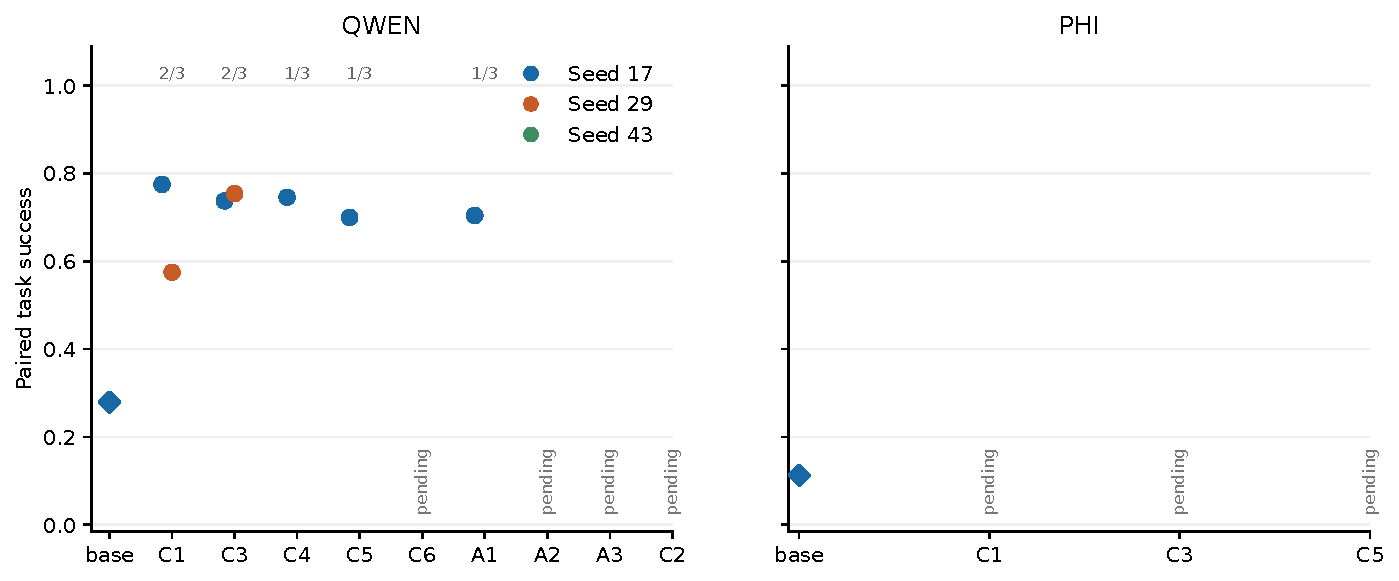
\includegraphics[width=\textwidth]{../reports/overnight_20261024T023622Z/figures/paired_success.pdf}
\caption{Antagonist-free 64-turn paired success on 240 families. Individual actual
seed values are shown; unavailable cells remain pending. The untrained diamond is
one shared reference per architecture. No error bars are inferred for missing seeds.}
\end{figure}
\begin{figure}[t]\centering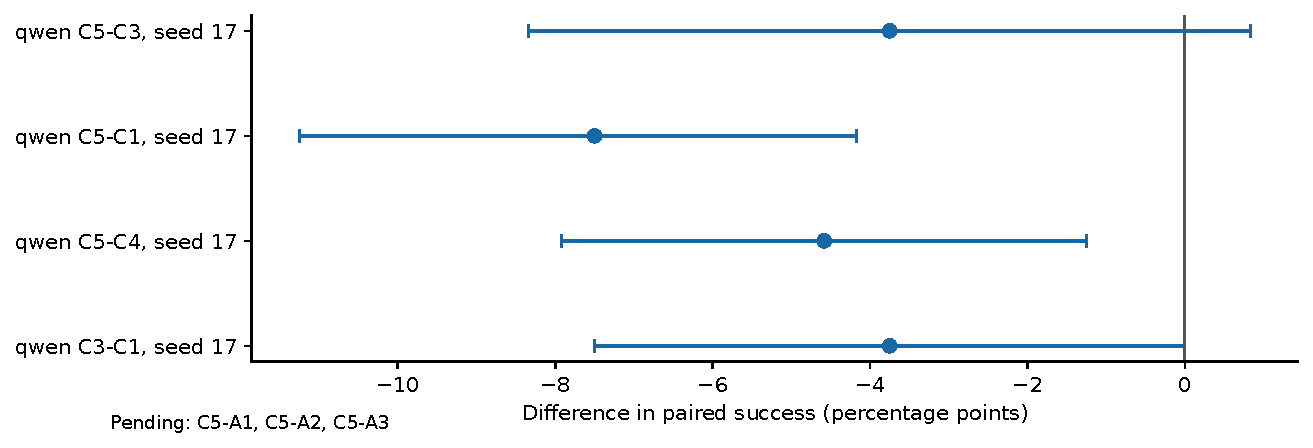
\includegraphics[width=\textwidth]{../reports/overnight_20261024T023622Z/figures/paired_contrasts.pdf}
\caption{Available individual-seed paired contrasts with exploratory 95\% family
bootstrap intervals. These intervals do not represent training-seed uncertainty.
Full planned-seed inference is reported separately when available.}
\end{figure}

\subsection{Failure structure and exposure}
Failure counts separate mutually exclusive categories and overlapping flags. They do not sum overlapping dependency, source and update errors as distinct failed conversations.
qwen C1 seed 17 has 90 failed conversations; all six commitments were recalled correctly in 471/480 conversations, and every canonical authorizing source was visible in 471/480 final prompts.
qwen C3 seed 17 has 99 failed conversations; all six commitments were recalled correctly in 472/480 conversations, and every canonical authorizing source was visible in 468/480 final prompts.
qwen C4 seed 17 has 98 failed conversations; all six commitments were recalled correctly in 463/480 conversations, and every canonical authorizing source was visible in 462/480 final prompts.
qwen C5 seed 17 has 118 failed conversations; all six commitments were recalled correctly in 444/480 conversations, and every canonical authorizing source was visible in 446/480 final prompts.
qwen A1 seed 17 has 111 failed conversations; all six commitments were recalled correctly in 467/480 conversations, and every canonical authorizing source was visible in 466/480 final prompts.
qwen C1 seed 29 has 167 failed conversations; all six commitments were recalled correctly in 464/480 conversations, and every canonical authorizing source was visible in 464/480 final prompts.
\begin{table}[ht]\centering\caption{Actual exposure across completed fits only; an unfinished second round must not be read as a full two-round budget.}\begin{tabular}{llrrr}\toprule Model & Condition & Seed & Training input tokens & Supervised targets\\\midrule
qwen & C1 & 17 & 2,097,152 & 97,683\\
qwen & C3 & 17 & 2,097,152 & 83,466\\
qwen & C4 & 17 & 2,097,152 & 78,417\\
qwen & C5 & 17 & 2,097,152 & 79,238\\
qwen & A1 & 17 & 2,097,152 & 80,051\\
qwen & C1 & 29 & 2,097,152 & 96,822\\
\bottomrule\end{tabular}\end{table}
Equal input-token quotas do not imply equal supervised-target exposure. These descriptive differences cannot establish that exposure caused performance differences.
C1 round-one recovery uses 14 distinct loss-contributing windows from 9 families on 363 contributing occurrences. The top five windows account for 37.4\% of recovery target tokens. Repetition does not create new independent examples.

\begin{figure}[t]\centering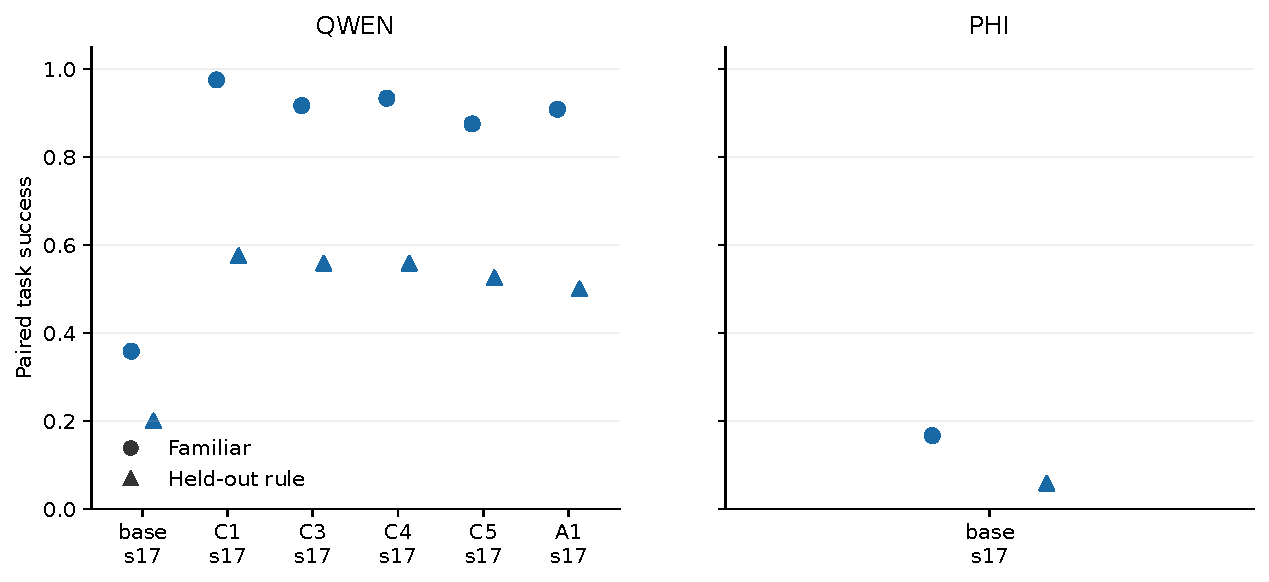
\includegraphics[width=\textwidth]{../reports/overnight_20261024T023622Z/figures/rule_structure.pdf}
\caption{Familiar and held-out-rule paired success, 120 families per stratum,
with completed model/seed values only. Domain and ambiguity limitations remain.}
\end{figure}
\begin{figure}[t]\centering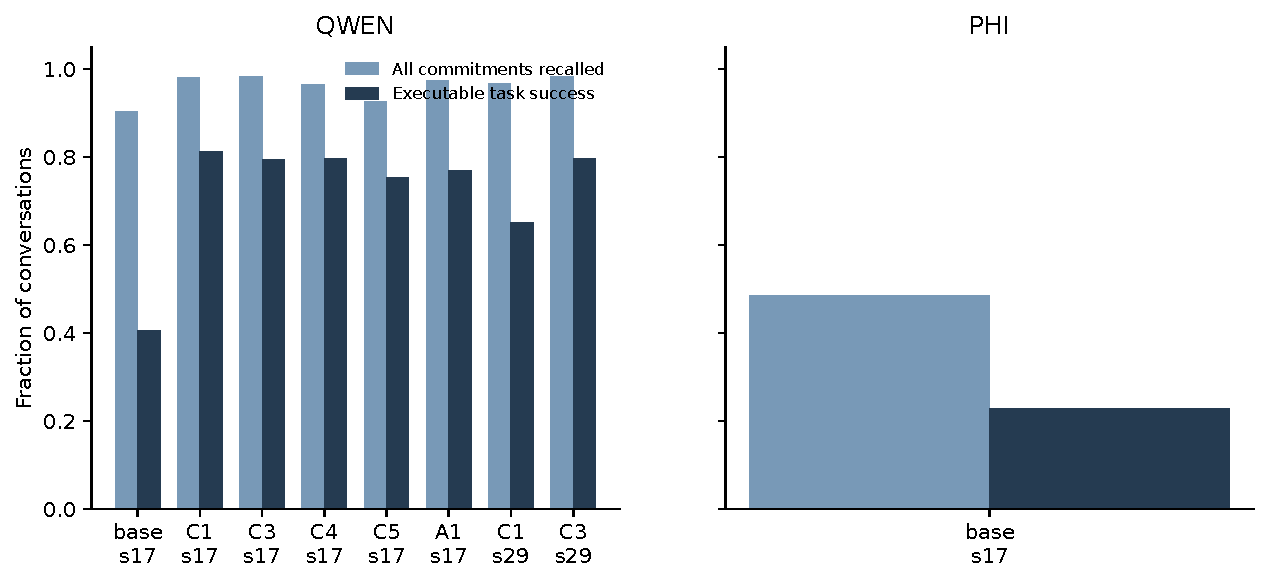
\includegraphics[width=\textwidth]{../reports/overnight_20261024T023622Z/figures/recall_behavior.pdf}
\caption{Correct recall of all six commitments versus correct executable behavior
on the same 480 conversations per seed. Descriptive bars do not treat worlds as
independent experimental units.}
\end{figure}
\begin{figure}[t]\centering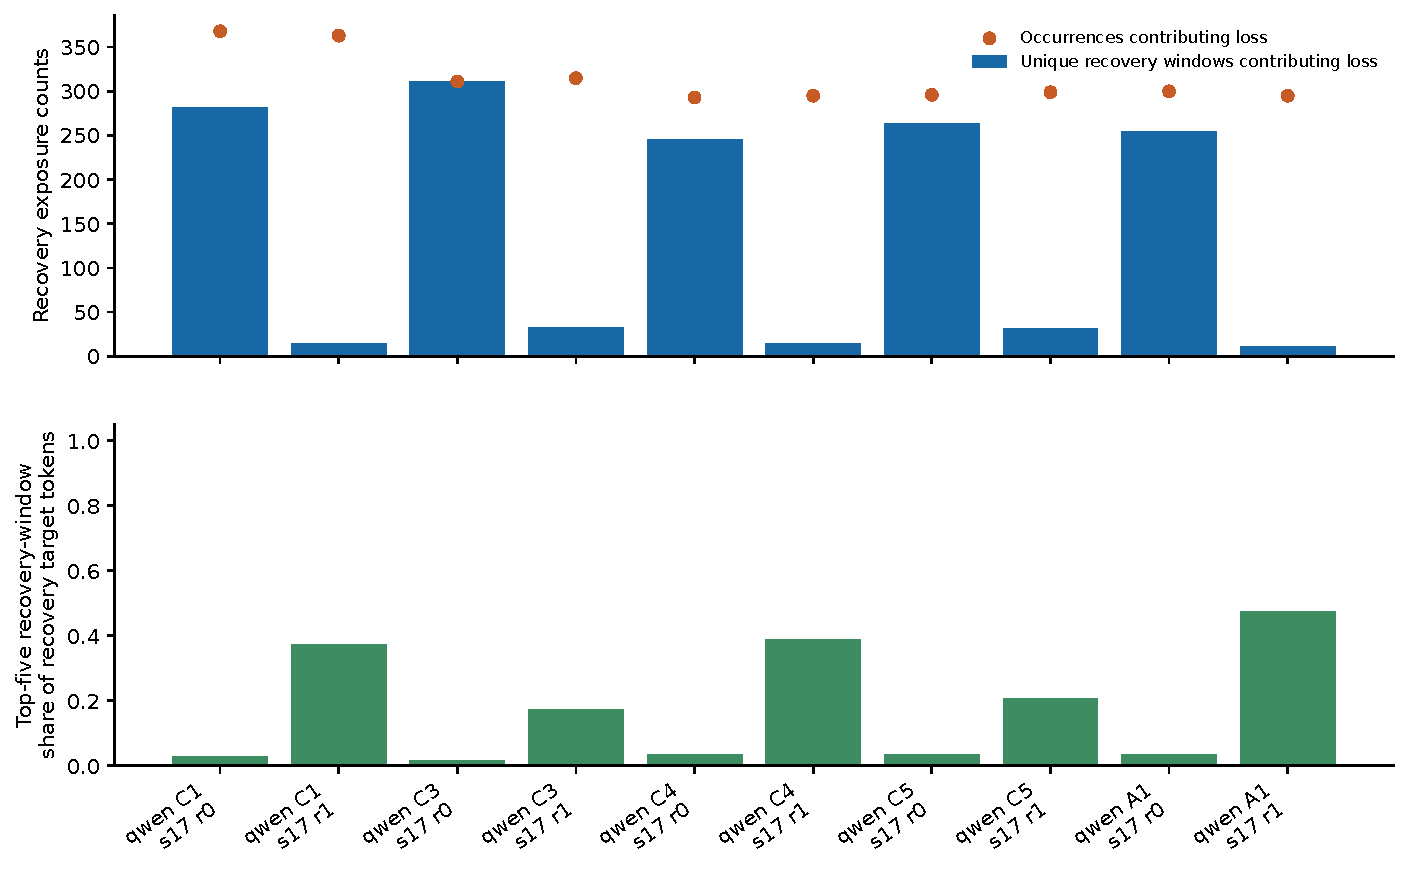
\includegraphics[width=\textwidth]{../reports/overnight_20261024T023622Z/figures/recovery_exposure.pdf}
\caption{Actual loss-contributing recovery windows, repeated occurrences and
concentration of target-token exposure. Loaded buffer windows are not automatically
counted as optimized examples.}
\end{figure}

\section{Post-review diagnostics and human validation}
Review supplement 001 was designed after C1 and the available C3 seed-17 result
were inspected. Its scientific code and protocol have a separate hash freeze.
It cannot run before all 241 core stages complete. It has at most two aggregate
reserved GPU-hours within the original 96-hour ceiling, preserving a half-hour
contingency. Timing-only profiling determines the frozen feasible allocation;
outcomes cannot change that allocation. None of these analyses is original
preregistered confirmation.
No supplementary GPU results are available in this draft; execution remains
pending the full-core gate.

A0 replays each checkpoint's own final prompt; A1 clears explicit working memory;
A2 additionally removes supplied assistant-authored sources while preserving the
remaining user sources and indices. Intact replay agreement must be examined
before interpreting differences. Similar terminal performance does not show that
memory never mattered earlier. Removed assistant evidence and source availability
must accompany any interpretation. A common user-only input reference, if admitted,
is collapsed source reasoning rather than a matched 64-turn rollout.

The fresh mechanism study uses incompatible Hyde/Rival options on the same slot,
contrasted with original separate-slot ownership, peer-disabled delivery and
motive-only representation. Policies are frozen, so it measures behavior, not a
learned-transfer benefit. Typed message/action matches and repeated coordination
candidates are only screens for human semantic review. The original final pilot
had 64 delivered antagonist messages, zero typed followups and zero repeated
candidates. This neither proves semantic interaction absent nor establishes
rivalry. A separate routing control cannot retroactively repair the learned
character-count comparison.

The existing 60-item action packet contains actual historical pilot exchanges,
with preserved item identities and two blank independent rating forms. Action
ratings remain distinct from the planned 120-output prose packet, which requires
all specified natural-language validation outputs. Missing prose outputs are not
filled with pilot or alternative-condition examples. No synthetic human ratings
or unsolicited contact with raters is permitted. The external LongMemEval subset
and independent-family replication remain separate forms of evidence with their
original protocols and disclosed adaptations.

\section{Limitations and claims for author review}
The benchmark uses fixed scripts, a narrow shared categorical schema, and a
retriever that often exposes canonical sources at the final turn. These features
can make rule execution and source reasoning more important than long-term memory.
Correct recall does not guarantee correct behavior. Source visibility is measured
using gold annotations only after input construction, never to choose a favorable
test subset. Temporal associations between character actions and later errors can
also reflect authorized user changes; they are not causal attack-effect estimates.

Input-token matching does not equal exact FLOP or supervised-target matching.
Character-conditioned inputs can differ in length, recovery-pool diversity,
interference severity, repetition and available source evidence. These properties
are reported as associations, without rebalancing or retraining frozen arms.
Distinct owned slots and non-enforced original routing limit stronger relationship
or coalition claims. Some training traces contain typed coordination candidates;
these require semantic review and do not by themselves establish meaningful
coordination. Profile, persistence
and interaction controls must be interpreted on their own results.

\begin{table}[ht]\centering\caption{Claim-to-evidence boundaries for scientific author review.}\begin{tabular}{p{.24\textwidth}p{.68\textwidth}}\toprule Claim & Required evidence or limitation\\\midrule
Base improvement & Compare completed per-seed rows with the one reused untrained reference; this alone is ordinary supervised-learning evidence.\\
Clean-training superiority & Requires C5 versus C1. A C5 advantage over C3 alone is insufficient.\\
Generic-adversarial advantage & Requires the prespecified C5 versus C3 contrast, with all planned seeds for confirmatory interpretation.\\
Narrative, history, peers & Require A1, A2 and A3 respectively; no pooled persona label establishes these mechanisms.\\
Memory necessity & Terminal-memory removals and common-input reasoning are pending unless their separately frozen diagnostics finish.\\
Broad transfer & Domain framings share one six-slot schema. Independent architecture replication and external memory QA are distinct, bounded evidence.\\
\bottomrule\end{tabular}\end{table}


\section{Reproducibility and generative-AI disclosure}
Compact code, configurations, manifests, tables and figures are committed locally
on main. Bulk traces, tokenizers, adapters and optimizer states remain Git ignored
and are mirrored locally because the pod's overlay is not verified persistent
storage. Per-run revisions, hashes, source snapshots, model calls, tokens, GPU
reservation, sampled utilization and memory measurements are retained. Reservation
time includes loads and failures; sampled utilization and observed container
lifetime are not billing records. The actual hourly rate is unknown.

Codex assisted with implementation, execution monitoring, analysis code, source
retrieval and draft text under an author-directed research brief. Human authors
must critically review and own the scientific ideas, arguments, results and
conclusions, and revise the assistance disclosure accurately. This document is
not an unattended compliant final submission. Nothing has been pushed, published
or submitted. The current official-template copy and previously verified conference
requirements are retained; requirements must be rechecked before any submission.

\bibliographystyle{splncs03}\bibliography{references}
\end{document}
